\documentclass[tikz,border=10pt]{standalone}
% Shared look for every TikZ diagram. Load with % Shared look for every TikZ diagram. Load with % Shared look for every TikZ diagram. Load with \input{../../tools/tikz-style.tex}
\usepackage[T1]{fontenc}
\usepackage{lmodern}
\renewcommand{\sfdefault}{lmr}  % diagrams use the same serif as the text
\usetikzlibrary{arrows.meta, positioning, shapes.geometric, calc, fit, backgrounds}
\definecolor{cblue}{HTML}{4C78A8}
\definecolor{corange}{HTML}{F58518}
\definecolor{cgreen}{HTML}{54A24B}
\definecolor{cred}{HTML}{E45756}
\definecolor{cpurple}{HTML}{B279A2}
\definecolor{cgrey}{HTML}{6B6B6B}
\tikzset{
  every picture/.style={font=\sffamily, line width=1.2pt},
  box/.style={draw=#1, fill=#1!12, rounded corners=4pt, align=center, inner sep=7pt, minimum height=1.1cm},
  box/.default=cgrey,
  arrow/.style={-{Stealth[length=3mm]}, draw=cgrey, line width=1.4pt},
  title/.style={font=\sffamily\bfseries\Large},
  note/.style={font=\sffamily\small, text=cgrey, align=center},
}
\AtBeginDocument{\hyphenpenalty=10000 \exhyphenpenalty=10000}

\usepackage[T1]{fontenc}
\usepackage{lmodern}
\renewcommand{\sfdefault}{lmr}  % diagrams use the same serif as the text
\usetikzlibrary{arrows.meta, positioning, shapes.geometric, calc, fit, backgrounds}
\definecolor{cblue}{HTML}{4C78A8}
\definecolor{corange}{HTML}{F58518}
\definecolor{cgreen}{HTML}{54A24B}
\definecolor{cred}{HTML}{E45756}
\definecolor{cpurple}{HTML}{B279A2}
\definecolor{cgrey}{HTML}{6B6B6B}
\tikzset{
  every picture/.style={font=\sffamily, line width=1.2pt},
  box/.style={draw=#1, fill=#1!12, rounded corners=4pt, align=center, inner sep=7pt, minimum height=1.1cm},
  box/.default=cgrey,
  arrow/.style={-{Stealth[length=3mm]}, draw=cgrey, line width=1.4pt},
  title/.style={font=\sffamily\bfseries\Large},
  note/.style={font=\sffamily\small, text=cgrey, align=center},
}
\AtBeginDocument{\hyphenpenalty=10000 \exhyphenpenalty=10000}

\usepackage[T1]{fontenc}
\usepackage{lmodern}
\renewcommand{\sfdefault}{lmr}  % diagrams use the same serif as the text
\usetikzlibrary{arrows.meta, positioning, shapes.geometric, calc, fit, backgrounds}
\definecolor{cblue}{HTML}{4C78A8}
\definecolor{corange}{HTML}{F58518}
\definecolor{cgreen}{HTML}{54A24B}
\definecolor{cred}{HTML}{E45756}
\definecolor{cpurple}{HTML}{B279A2}
\definecolor{cgrey}{HTML}{6B6B6B}
\tikzset{
  every picture/.style={font=\sffamily, line width=1.2pt},
  box/.style={draw=#1, fill=#1!12, rounded corners=4pt, align=center, inner sep=7pt, minimum height=1.1cm},
  box/.default=cgrey,
  arrow/.style={-{Stealth[length=3mm]}, draw=cgrey, line width=1.4pt},
  title/.style={font=\sffamily\bfseries\Large},
  note/.style={font=\sffamily\small, text=cgrey, align=center},
}
\AtBeginDocument{\hyphenpenalty=10000 \exhyphenpenalty=10000}

\begin{document}
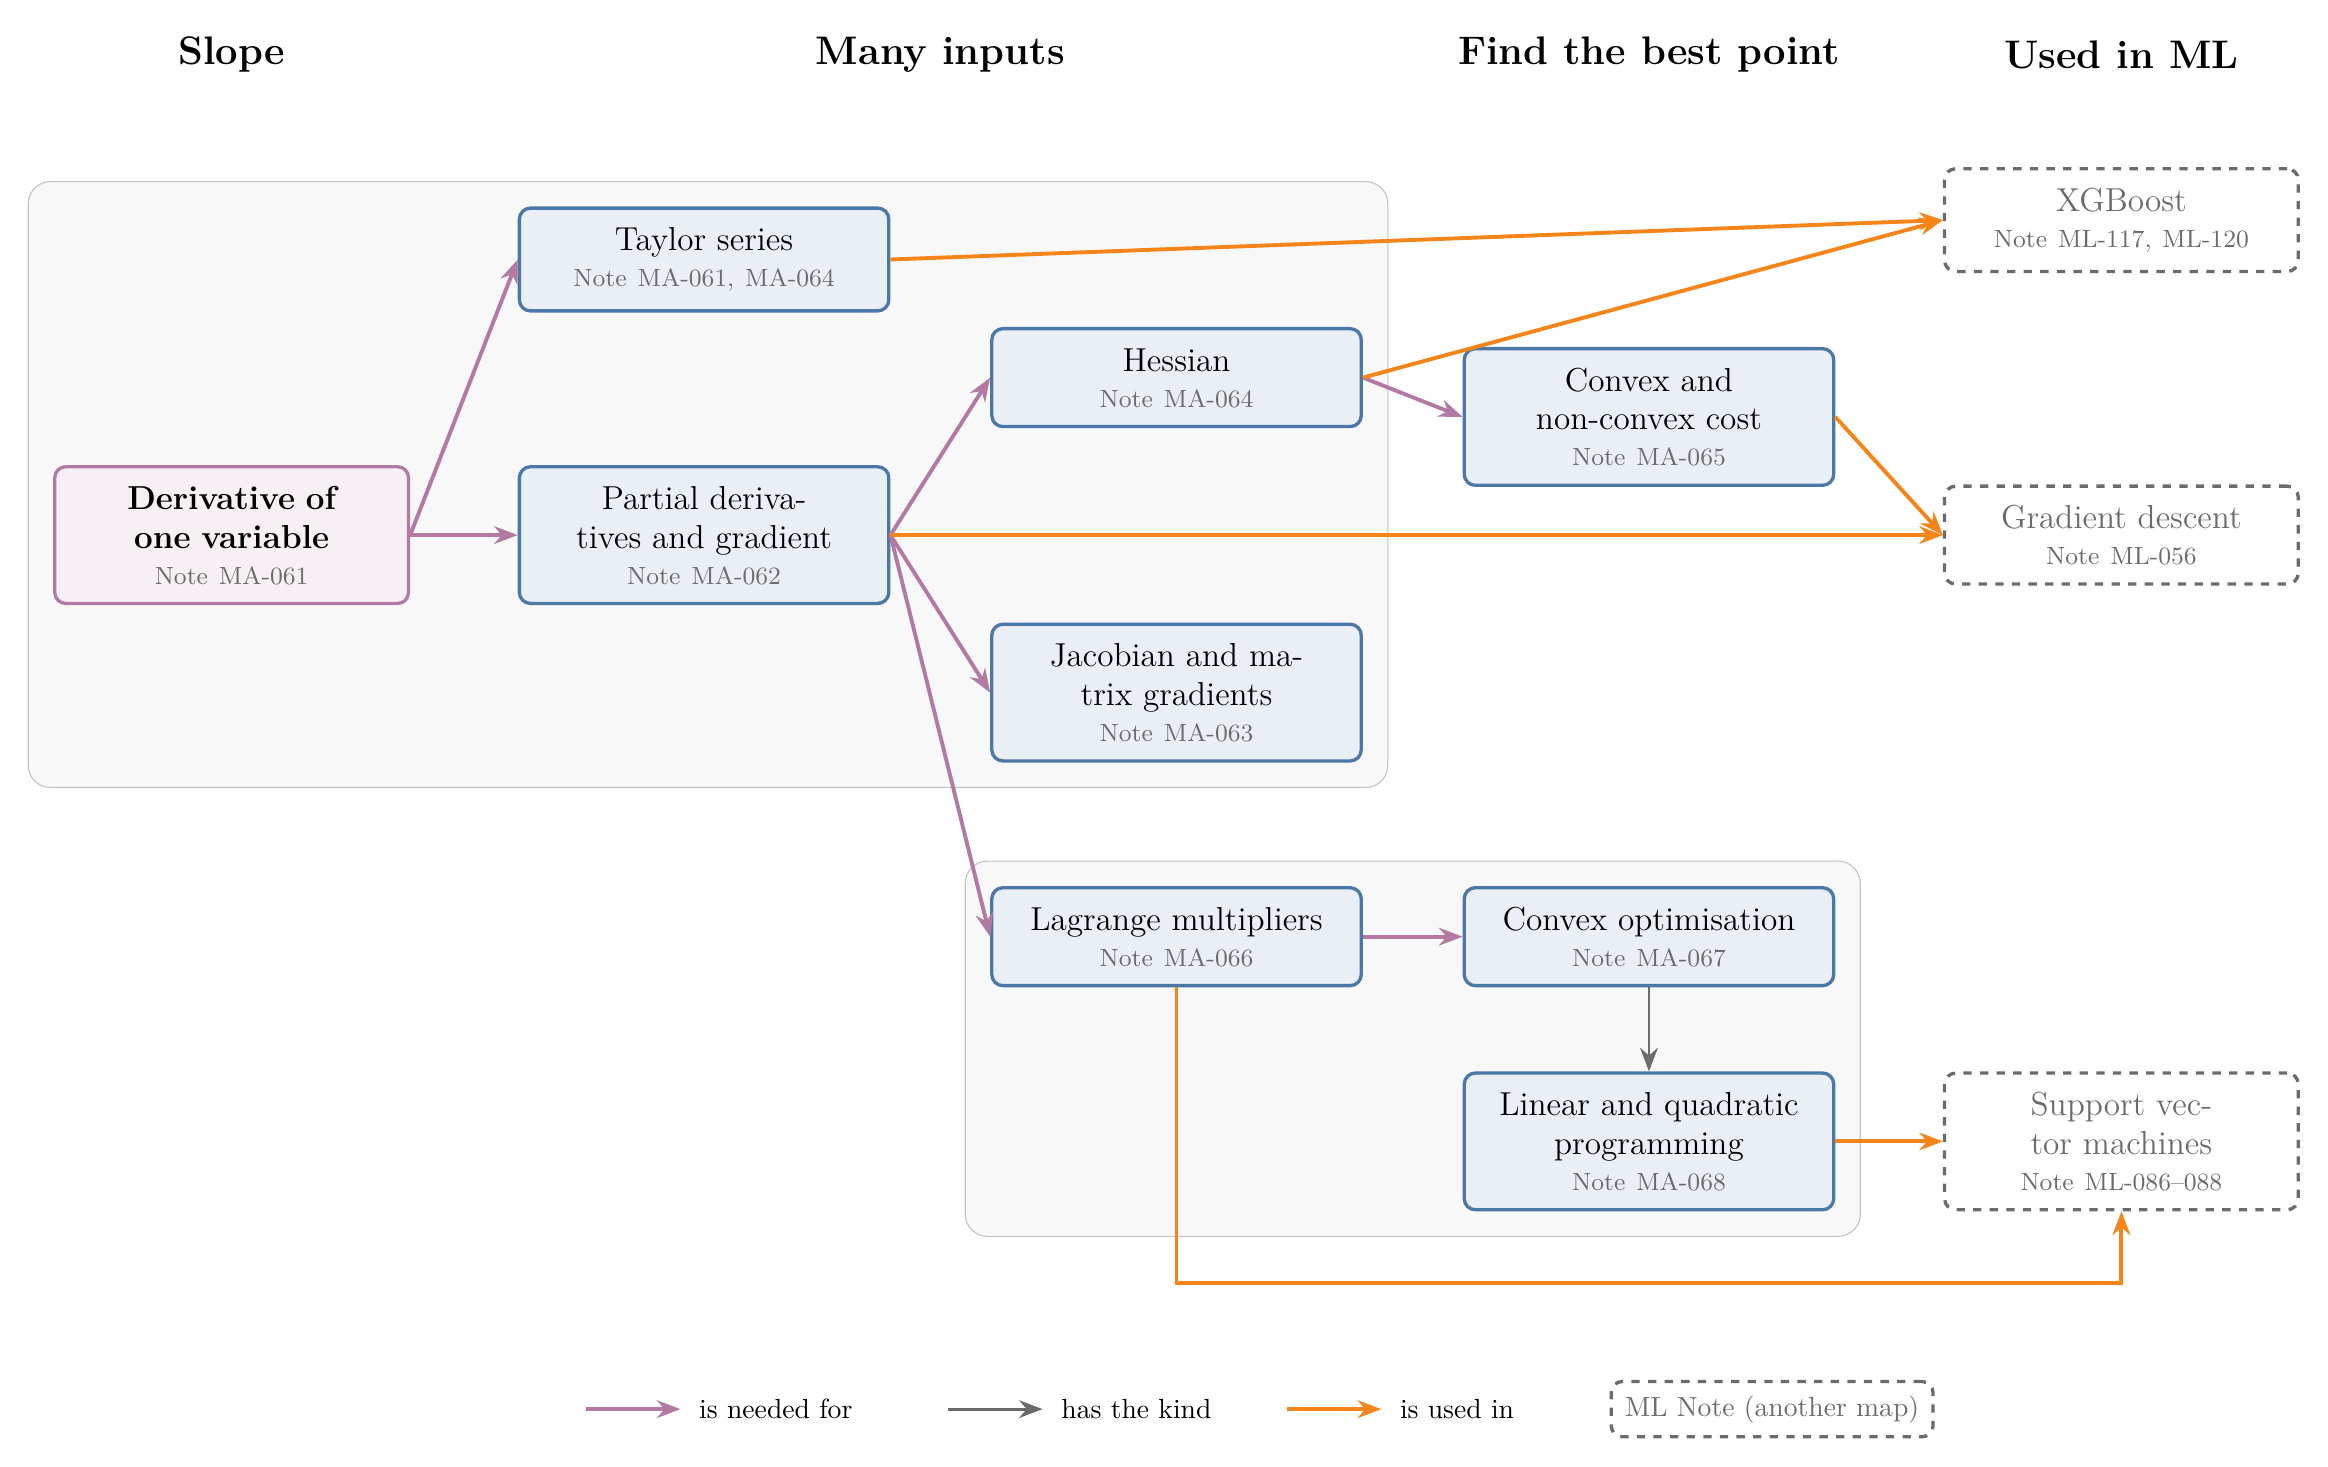
\begin{tikzpicture}[
    every node/.append style={font=\sffamily\large},
    idea/.style={box=cpurple, text width=4.0cm},
    con/.style={box=cblue, text width=4.2cm},
    prev/.style={draw=cgrey, dashed, rounded corners=4pt, align=center, inner sep=7pt, text=cgrey, text width=4.0cm, minimum height=1.1cm},
    group/.style={draw=cgrey!40, fill=cgrey!5, rounded corners=8pt, inner sep=9pt},
    needs/.style={arrow, draw=cpurple},
    kind/.style={arrow, draw=cgrey, line width=1pt},
    used/.style={arrow, draw=corange},
  ]
  \newcommand{\nt}[1]{\\[-1pt]{\small\color{cgrey}Note #1}}
  \node[title] at (0,10.6)  {Slope};
  \node[title] at (9,10.6)  {Many inputs};
  \node[title] at (18,10.6) {Find the best point};
  \node[title] at (24,10.6) {Used in ML};

  % ---- derivatives
  \node[idea] (der) at (0,4.5) {\textbf{Derivative of one variable}\nt{MA-061}};
  \node[con] (tay) at (6,8.0) {Taylor series\nt{MA-061, MA-064}};
  \node[con] (gra) at (6,4.5) {Partial derivatives and gradient\nt{MA-062}};
  \node[con] (hes) at (12,6.5) {Hessian\nt{MA-064}};
  \node[con] (jac) at (12,2.5) {Jacobian and matrix gradients\nt{MA-063}};

  % ---- optimisation
  \node[con] (cvx) at (18,6.0) {Convex and non-convex cost\nt{MA-065}};
  \node[con] (lag) at (12,-0.6) {Lagrange multipliers\nt{MA-066}};
  \node[con] (cop) at (18,-0.6) {Convex optimisation\nt{MA-067}};
  \node[con] (lp)  at (18,-3.2) {Linear and quadratic programming\nt{MA-068}};

  % ---- ML uses
  \node[prev] (xgb) at (24,8.5)  {XGBoost\nt{ML-117, ML-120}};
  \node[prev] (gd)  at (24,4.5)  {Gradient descent\nt{ML-056}};
  \node[prev] (svm) at (24,-3.2) {Support vector machines\nt{ML-086--088}};

  \begin{scope}[on background layer]
    \node[group, fit=(der) (tay) (gra) (hes) (jac)] {};
    \node[group, fit=(lag) (cop) (lp)] {};
  \end{scope}

  \draw[needs] (der.east) -- (tay.west);
  \draw[needs] (der.east) -- (gra.west);
  \draw[needs] (gra.east) -- (hes.west);
  \draw[needs] (gra.east) -- (jac.west);
  \draw[needs] (gra.east) -- (lag.west);
  \draw[needs] (hes.east) -- (cvx.west);
  \draw[used]  (tay.east) -- (xgb.west);
  \draw[used]  (hes.east) -- (xgb.west);
  \draw[used]  (gra.east) -- (gd.west);
  \draw[used]  (cvx.east) -- (gd.west);
  \draw[needs] (lag.east) -- (cop.west);
  \draw[kind]  (cop.south) -- (lp.north);
  \draw[used]  (lp.east) -- (svm.west);
  \draw[used]  (lag.south) -- (12,-5.0) -| (svm.south);

  % legend
  \begin{scope}[shift={(4.5,-6.6)}, every node/.style={font=\sffamily, anchor=west}]
    \draw[needs] (0,0) -- (1.2,0);     \node at (1.3,0) {is needed for};
    \draw[kind] (4.6,0) -- (5.8,0);    \node at (5.9,0) {has the kind};
    \draw[used] (8.9,0) -- (10.1,0);   \node at (10.2,0) {is used in};
    \node[draw=cgrey, dashed, rounded corners=4pt, inner sep=5pt, text=cgrey, anchor=west] at (13.0,0) {ML Note (another map)};
  \end{scope}
\end{tikzpicture}
\end{document}
